
%(BEGIN_QUESTION)
% Copyright 2008, Tony R. Kuphaldt, released under the Creative Commons Attribution License (v 1.0)
% This means you may do almost anything with this work of mine, so long as you give me proper credit

En av de mest grunnleggende komponentene i et pneumatisk instrument er den såkalte \textit{flapper/nozzle}- eller \textit{baffle/nozzle}-enheten.  Den består av to strupinger i luftstrømmen: én inne i et rør (\textit{orifice}) og én ved enden av et rør (\textit{nozzle}).  \textit{Flapper} eller \textit{baffle} er i praksis bare en flat metallbit som ligger tett ved dysetuppen.  Disse mekanismene fungerer som svært følsomme posisjonsdetektorer, og genererer et pneumatisk utgangssignal som varierer med flapper- (baffle-)posisjon:

$$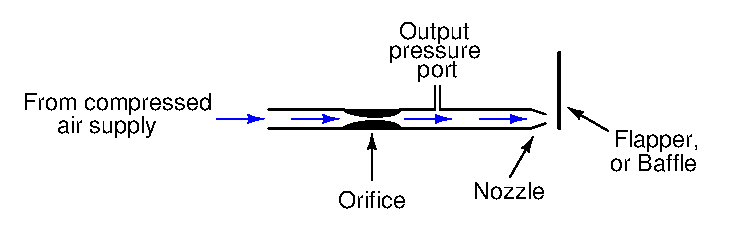
\includegraphics[width=15.5cm]{i00191x01.eps}$$

Anta at to trykkmålere installeres langs røret, én oppstrøms for orifice og én nedstrøms for orifice, slik:

$$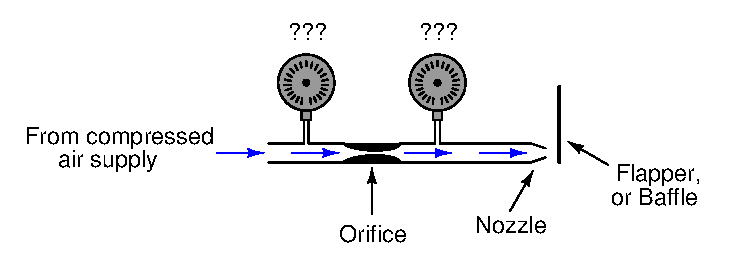
\includegraphics[width=15.5cm]{i00191x02.eps}$$

Hva vil disse to trykkmålerne vise kvalitativt sett?  Anta at lufttilførselen reguleres av en trykkregulator og dermed holder konstant trykk.  Vil de to målerne vise samme trykk?  Vil den ene vise høyere trykk enn den andre?  Forklar svaret.

\vskip 10pt

Hvis flapperen (baffle) flyttes nærmere dysen, blir dysen mer strupende for luftstrømmen.  Hvilken effekt får dette på de to trykkmålerne i dette flapper/nozzle-systemet?

$$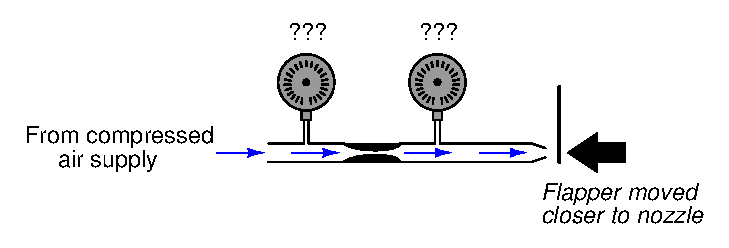
\includegraphics[width=15.5cm]{i00191x03.eps}$$

\vskip 10pt

Hvis flapperen flyttes lengre vekk fra dysen, hvilken effekt får det på de to trykkmålernes avlesning?

$$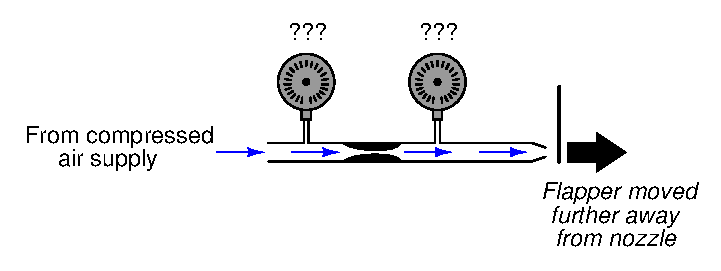
\includegraphics[width=15.5cm]{i00191x04.eps}$$

\underbar{file i00191}
%(END_QUESTION)





%(BEGIN_ANSWER)

Trykkmåleren nedstrøms for orifice vil vise lavere trykk enn måleren oppstrøms for orifice.  Når flapperen flyttes nærmere dysen, øker nedstrømstrykket.  Når flapperen flyttes bort fra dysen, reduseres nedstrømstrykket.

\vskip 10pt

Oppfølgingsspørsmål: tegn et skjematisk diagram av en elektrisk krets som er analog med denne pneumatiske ``kretsen'' dannet av trykkilde, orifice, dyse og flapper.

%(END_ANSWER)





%(BEGIN_NOTES)

Trykket oppstrøms vil i praksis forbli konstant, slik det holdes av trykkregulatoren oppstrøms.

\vskip 10pt

Oppfølgingssvar:

$$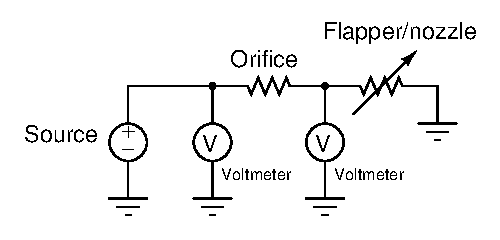
\includegraphics[width=15.5cm]{i00191x05.eps}$$

%INDEX% Basics, pneumatics: baffle/nozzle
%INDEX% Basics, pneumatics: flapper/nozzle

%(END_NOTES)

